
\documentclass{beamer}

\mode<presentation> {


\usetheme{Montpellier}

% As well as themes, the Beamer class has a number of color themes
% for any slide theme. Uncomment each of these in turn to see how it
% changes the colors of your current slide theme.

\usecolortheme{beaver}


%\setbeamertemplate{footline} % To remove the footer line in all slides uncomment this line
\setbeamertemplate{footline}[page number] % To replace the footer line in all slides with a simple slide count uncomment this line

\setbeamertemplate{navigation symbols}{} % To remove the navigation symbols from the bottom of all slides uncomment this line
}

\usepackage{graphicx} % Allows including images
\usepackage{booktabs} % Allows the use of \toprule, \midrule and \bottomrule in tables
\usepackage{amsmath}
\usepackage{lmodern}% http://ctan.org/pkg/lm
\newenvironment{where}{\noindent{}where\begin{itemize}}{\end{itemize}}
\DeclareMathOperator{\Exists}{\exists}
%----------------------------------------------------------------------------------------
%	TITLE PAGE
%----------------------------------------------------------------------------------------

\title[Exit Exam]{Fast Dictionary Attacks on Passwords Using Time-Space Tradeoff} % The short title appears at the bottom of every slide, the full title is only on the title page

\author{Tyler Combs} % Your name
\institute[OU] % Your institution as it will appear on the bottom of every slide, may be shorthand to save space
{
The University of Oklahoma \\ % Your institution for the title page
\medskip
\textit{tyler.combs@ou.edu} % Your email address
}
\date{April 14, 2015} % Date, can be changed to a custom date

\begin{document}

\begin{frame}
\titlepage % Print the title page as the first slide
\end{frame}

\begin{frame}
\frametitle{Overview} % Table of contents slide, comment this block out to remove it
\tableofcontents % Throughout your presentation, if you choose to use \section{} and \subsection{} commands, these will automatically be printed on this slide as an overview of your presentation
\end{frame}

%----------------------------------------------------------------------------------------
%	PRESENTATION SLIDES
%----------------------------------------------------------------------------------------

%------------------------------------------------
\section{Introduction} 
%------------------------------------------------
\subsection{What is the problem?}
\begin{frame}
\frametitle{What is the problem?}
$
P(\alpha) = \prod_{x \in \alpha} \mathcal{V}(x)
$
\end{frame}



\subsection{Dictionary Attacks}
\begin{frame}
\frametitle{Dictionary Attacks}
\end{frame}

\subsection{Previous Work}
\begin{frame}
\frametitle{Helman}
\end{frame}

\begin{frame}
\frametitle{Rainbow}
\end{frame}

%------------------------------------------------
\section{Filtering} 
%------------------------------------------------
\subsection{Markovian}

\begin{frame}
\frametitle{Markov Chains}
\begin{itemize}
\item Markov chains are commonly used in natural language processing. Most notably speech recognition systems.
\item Markov models have been used to generate passwords for users.
\item Given a set of states $S = \lbrace s_1,s_2,\dotsb,s_n \rbrace$ there is some probability $p_{ij}$ that denotes the probability of transitioning from state $s_i$ to state $s_j$
\item The probability of transitioning to the next state depends only on the current state
\end{itemize}
\end{frame}

\begin{frame}
\frametitle{Markov Chains}

\textbf{The order of a Markov chain of order n is defined as:}
\begin{align*}
& P(X_n = x_n | X_{n-1} = x_{n-1}, X_{n-2} = x_{n-2}, \dotsb , X_1 = x_1) = \\ & P(X_n = x_n | X_{n-1} = x_{n-1}, \dotsb , X_{n-m} = x_{n-m})
\end{align*}

\textbf{Zero-order Markov Chain:}
\begin{align*}
& P(X_n = x_n | X_{n-1} = x_{n-1}, X_{n-2} = x_{n-2}, \dotsb , X_1 = x_1) =  \\ & P(X_n = x_n)
\end{align*}

\textbf{First-order Markov Chain:}
\begin{align*}
& P(X_n = x_n | X_{n-1} = x_{n-1}, X_{n-2} = x_{n-2}, \dotsb , X_1 = x_1) = \\ & P(X_n = x_n | X_{n-1} = x_{n-1})
\end{align*}
\end{frame}

\begin{frame}
\frametitle{Zero-order Markov Model}
In a zero-order Markov model, each character is generated given its underlying proability distribution. This is based on the frequency of the letter in the users natural language. Formally the zero-order model can be written as:
\begin{equation*}
P(\alpha) = \prod_{x \in \alpha} \mathcal{V}(x)
\end{equation*}
where:
\begin{where}
\item $P(\cdot)$ is the markovian proability distrubuion
\item $\alpha$ is a string of characacters
\item $\mathcal{V(\cdot)}$ is the frequency of a letter occuring in English
\item $x$ is an individual character
\end{where}
\end{frame}


\begin{frame}
\frametitle{First-order Markov Model}

In a First-order Markov model, each ordered pair is assigned a proability and each character is generated by looking at the pervious character. The first-order markov model can be written as:
\begin{equation*}
P(x_1x_2x_3 \dotsb x_n) = \mathcal{V}(x_1)\prod_{i=1}^{n-1}\mathcal{V}(x_{i+1}|x_i)
\end{equation*}
where:
\begin{where}
\item $P(\cdot)$ is the markovian proability distrubuion
\item $x_i$ are individual characters
\item $\mathcal{V(\cdot)}$ is the frequency of a letter or ordered pair occuring in English
\end{where}
\end{frame}



\begin{frame}
\frametitle{Markov Dictionary}
A probability distribution is not a dictionary. To create a dictionary, discretize the probabilities into two levels using a threshold $\theta$
\begin{block}{Zero-order dictionary}
\begin{equation*}
\mathcal{D}_{\mathcal{V},\theta} = \lbrace \alpha : \prod_{x \in \alpha}\mathcal{V}(x) \geq \theta \rbrace
\end{equation*}
\end{block}

\begin{block}{First-order dictionary}
\begin{equation*}
\mathcal{D}_{\mathcal{V},\theta} = \lbrace x_1x_2 \dotsb x_n : \mathcal{V}(x_1) \prod_{i = 1}^{n-1} \mathcal{V}(x_{i+1}|x_i) \geq \theta \rbrace
\end{equation*}
\end{block}
\end{frame}

\begin{frame}
\frametitle{Markov Dictionary}
The zero-order model is better for abrivtations and acrynyms. For example, a user picks their favorite song lyric and the first letter of each word creates their password.
\begin{figure}
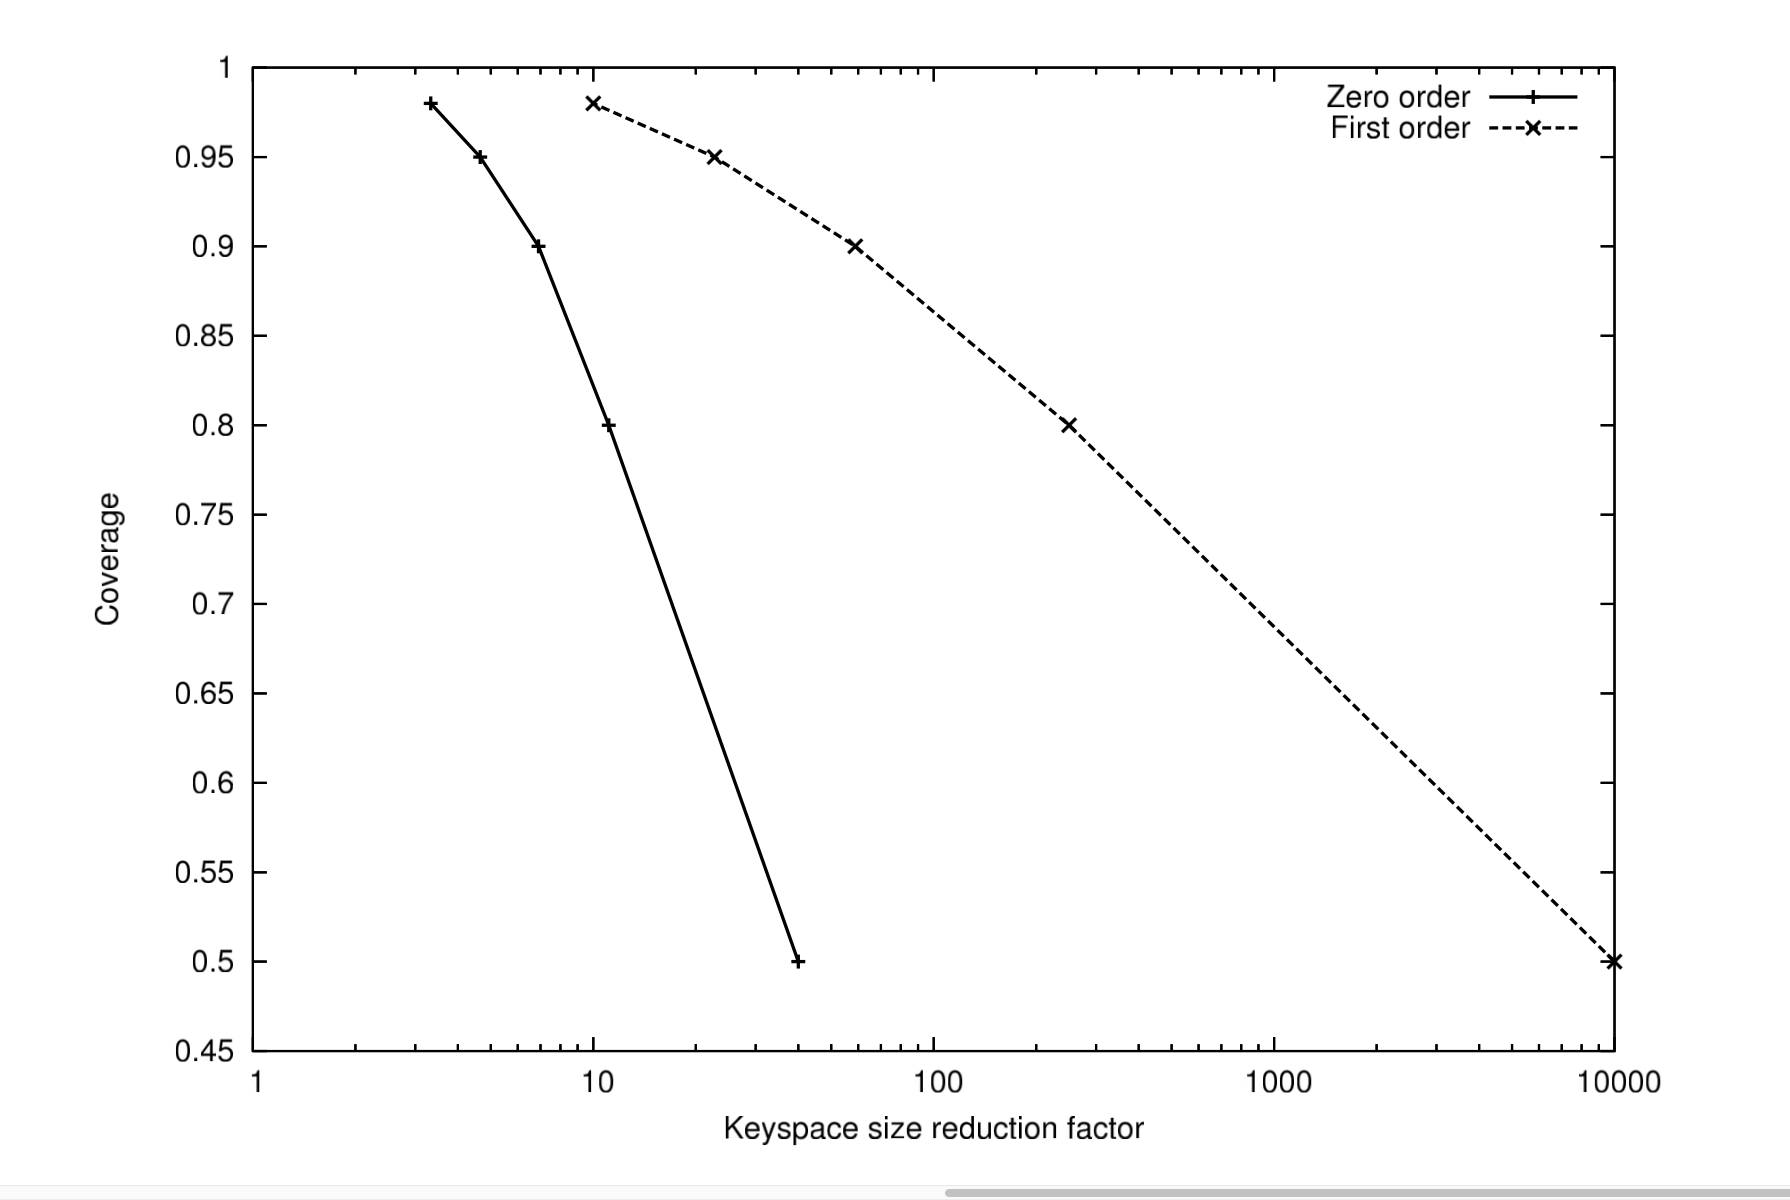
\includegraphics[width=0.6\linewidth]{figs/dict_plot}
\caption{Convergence vs reduction in Keyspace size ($|\mathcal{K}|$) for 8-character sequences}
\end{figure}
\end{frame}

\subsection{Finite Automaton}
\begin{frame}
\frametitle{Deterministic Finite Automaton}
\begin{itemize}
\item A DFA or Deterministic Finite Automaton is a finite state machine that accepts or rejects a string
\item A regular expression can be constructed from a DFA
\item Humans are not random with how they use numerals and special characters
\begin{itemize}
\item Numbers tend to be at the end of a password: password1
\item Capital letters are typically at the begining of a password: Password
\item there are typically more lowercase letters in passwords than uppercase letters, numerals, or special characters
\end{itemize}
\end{itemize}
\end{frame}

\begin{frame}
\frametitle{Dictionary using a DFA} 
An improved dictionary is one where strings are both accepted by a Markovian filter and accepted by at least one DFA from some set of DFA's. The updated dictionary is defined as:
\begin{equation*}
\mathcal{D}_{\mathcal{V},\theta,\langle M_i \rangle} = \lbrace \alpha : \prod_{x \in \alpha}\mathcal{V}(x) \geq \theta, and \Exists i : M_i accepts \alpha \rbrace
\end{equation*}
\begin{where}
\item $A$ is the set of 26 uppercase characters
\item $a$ is the set of 26 lowercase characters
\item $n$ is the set if 10 numerals
\item $s$ is the set of 5 special characters $\lbrace space, hyphen, underscore, period, comma \rbrace$
\end{where}

\end{frame}

%------------------------------------------------
\section{Indexing Algorithms} 
%------------------------------------------------
\begin{frame}
\frametitle{Indexing Algorithms}
\begin{itemize}
\item The goal is to create an algorithm that will efficiently enumerate the passwords in a given password space. Given $i$ as input return the $i^{th}$
\item In the rainbow attack the reduction function maps from ciphertext space to $\lbrace 0, 1, \dotsb, \lvert \mathcal{K} - 1 \rvert \rbrace$
\item Composed with a mapping from $\lbrace 0, 1, \dotsb, \lvert \mathcal{K}-1 \rvert \rbrace$ to a key in $\mathcal{K}$.
\item Makes no assumption about keyspace other than its size
\item Use the rainbow attack with a "smart" way to choose the keyspace
\end{itemize}
\end{frame}

\begin{frame}
\frametitle{Dictionary Modification}
Modify the dictionary to only consider fixed length strings. This allows for different threshold values $\theta$ for each length.
\begin{equation*}
\mathcal{D}_{\mathcal{V},\theta,\ell} = \lbrace \alpha :  \lvert \alpha \rvert = \ell and \prod_{x \in \alpha}\mathcal{V}(x) \geq \theta \rbrace
\end{equation*}
\end{frame}

\begin{frame}
\frametitle{Discretization}
The algorithm also needs to discretize the probability distribution of the strings. First, turn the dictionary into a sum rather than a product. \\
Transform the product
\begin{align*}
\prod_{x \in \alpha}\mathcal{V}(x) & \geq \theta \\
\log(\prod_{x \in \alpha}\mathcal{V}(x)) & \geq \log(\theta) \\
\log(\mathcal{V}(x_1)\mathcal{V}(x_2)\dotsb \mathcal{V}(x_n)) & \geq \log(\theta) \\
\log(\mathcal{V}(x_1)) + \log(\mathcal{V}(x_2)) + \dotsb + log(\mathcal{V}(x_n)) & \geq \log(\theta)
\end{align*}
\end{frame}

\begin{frame}
\frametitle{Discretization}
To arrive at a discrete version of the modified dictionary:
\begin{equation*}
\mathcal{D}_{\mathcal{V},\theta,\ell} = \lbrace \alpha :  \lvert \alpha \rvert = \ell and \sum_{x \in \alpha}\mu(x) \geq \lambda \rbrace
\end{equation*}
Where
\begin{where}
\item $\mu(x) = \log(\mathcal{V}(x))$
\item $\lambda = \log(\theta)$ 
\end{where}
\end{frame}

\begin{frame}
\frametitle{Discretization}
\begin{itemize}
\item $\mu(x) = \log(\mathcal{V}(x))$
\item Discretize the values of the $\mu$ function to the nearest multiple of some $\mu_0$
\item Narayanan and Shmatikov use a $\mu_0$ that yields approximately 1000 different discrete values
\end{itemize}
\end{frame}

\begin{frame}
\frametitle{Zero-Order Markovian Dictionary}
\end{frame}
\begin{frame}
\frametitle{First-Order Markovian Dictionary}
\end{frame}
\begin{frame}
\frametitle{DFA Dictionary}
\end{frame}
\begin{frame}
\frametitle{Any Keyspace $\mathcal{K}$}
\end{frame}
\begin{frame}
\frametitle{Hybrid Markovian/DFA}
\end{frame}
\begin{frame}
\frametitle{Multiple Keyspaces}
\end{frame}
\begin{frame}
\frametitle{Optimizations}
\end{frame}

%------------------------------------------------
\section{Experiment} 
%------------------------------------------------
\begin{frame}
\frametitle{Experiment}
\begin{itemize}
\item Measure coverage of rainbow attack vs hybrid attack
\item 142 real user passwords
\item 6-Character alphanumeric sequences for the rainbow attack ($|\mathcal{K}| = 36^6 \approx 2*10^9 $)
\item 70 regular expressions
\end{itemize}
\end{frame}

\begin{frame}
\frametitle{Results}
\begin{figure}
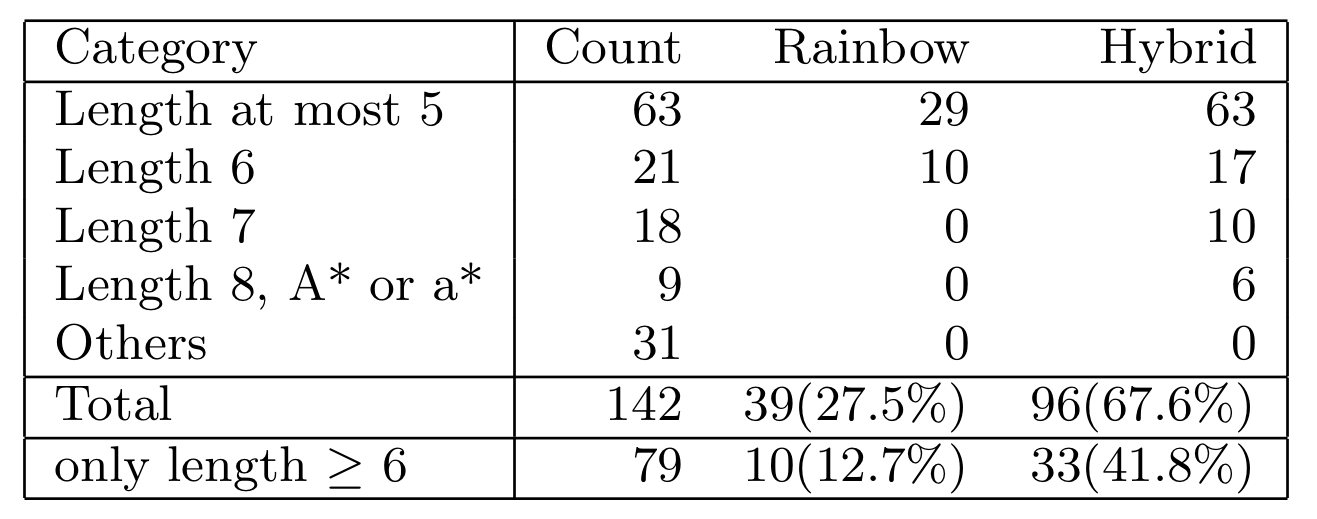
\includegraphics[width=0.9\linewidth]{figs/results}
\caption{Passwords recovered in Hybrid attack vs. Rainbow attack}
\end{figure}
\end{frame}

%------------------------------------------------
\section{Conclusions} 
%------------------------------------------------

\begin{frame}
\frametitle{Conclusions}
\begin{itemize}
\item One of many attacks targeting human weakness
\item Some possible defences against dictionary attacks for human memorable passwords
\begin{itemize}
\item Graphical passwords
\item Biometric information
\end{itemize}
\item Are these actually safer?
\end{itemize}
\end{frame}


%------------------------------------------------
\section{Analysis} 
%------------------------------------------------
\begin{frame}
\frametitle{Analysis}

\end{frame}




\end{document} 